\section{Experiments}
\label{sec:experiments}

We evaluate WuYa on two primary tasks: submission recommendation and journal review. This section describes the experimental setup, results, and ablation studies.

\subsection{Experimental Setup}

\subsubsection{Datasets}

We construct a benchmark dataset of 5,000 papers from five disciplines:
\begin{itemize}
    \item \textbf{Computer Science} (1,500 papers): From arXiv CS.AI, CS.CL, CS.LG, published 2022-2024.
    \item \textbf{Biology} (1,000 papers): From bioRxiv, selected from high-citation papers.
    \item \textbf{Economics} (1,000 papers): From NBER working papers and top economics journals.
    \item \textbf{Physics} (1,000 papers): From arXiv physics, selected from Q1 journal publications.
    \item \textbf{Medicine} (500 papers): From PubMed Central, RCT papers only.
\end{itemize}

Each paper is annotated with:
\begin{itemize}
    \item Publication venue and its tier (Q1-Q4, A-D).
    \item Five-dimensional evaluation scores by two expert human reviewers (inter-rater reliability $\kappa = 0.78$).
    \item Editor/reviewer feedback from actual review processes (where available).
\end{itemize}

\subsubsection{Evaluation Metrics}

For \textbf{submission recommendation}:
\begin{itemize}
    \item Top-1, Top-3, Top-5 accuracy: Whether the correct journal tier appears in the top-1/3/5 recommendations.
    \item Mean Reciprocal Rank (MRR): Position of the correct tier in the recommendation list.
\end{itemize}

For \textbf{journal review}:
\begin{itemize}
    \item Spearman correlation: Between WuYa's evaluation scores and human expert ratings.
    \item Kendall's tau: Pairwise agreement between WuYa and experts.
    \item Mean Absolute Error (MAE): Absolute difference in overall quality scores.
\end{itemize}

For \textbf{self-improvement}:
\begin{itemize}
    \item Frontier accuracy: Whether learned frontier surfaces match actual journal preferences.
    \item Improvement rate: Change in recommendation accuracy as frontier library grows.
\end{itemize}

\subsection{Baseline Methods}

We compare WuYa against the following baselines:

\begin{itemize}
    \item \textbf{Pure LLM}: GPT-4 with zero-shot evaluation, no retrieval or prior calibration.
    \item \textbf{Rule-Based}: Expert-defined rules mapping scoring dimensions to tiers without LLM or prior.
    \item \textbf{Citation-Only}: Recommendation based solely on citation network features.
    \item \textbf{PaperDigest}: Existing academic paper analysis tool \citep{kang2018peerread}.
    \item \textbf{WuYa w/o Self-Improvement}: Our system without the frontier discovery mechanism.
\end{itemize}

\subsection{Main Results}

\subsubsection{Submission Recommendation}

Table~\ref{tab:recommendation-results} shows submission recommendation accuracy across disciplines.

\begin{table}[t]
\centering
\caption{Submission Recommendation Accuracy (Top-K) by Discipline}
\label{tab:recommendation-results}
\begin{tabular}{@{}lcccccc@{}}
\toprule
\textbf{Method} & \textbf{CS} & \textbf{Bio} & \textbf{Econ} & \textbf{Physics} & \textbf{Med} & \textbf{Avg} \\
\midrule
Pure LLM & 52.1 & 48.3 & 45.7 & 51.2 & 49.8 & 49.4 \\
Rule-Based & 41.2 & 39.8 & 38.5 & 42.1 & 40.3 & 40.4 \\
Citation-Only & 38.7 & 35.2 & 33.1 & 36.9 & 34.8 & 35.7 \\
PaperDigest & 45.3 & 42.1 & 40.2 & 43.8 & 41.5 & 42.6 \\
WuYa w/o SI & 68.2 & 64.5 & 61.3 & 67.1 & 65.8 & 65.4 \\
\textbf{WuYa (full)} & \textbf{73.8} & \textbf{69.2} & \textbf{66.1} & \textbf{72.5} & \textbf{70.1} & \textbf{70.3} \\
\bottomrule
\end{tabular}
\end{table}

WuYa achieves 70.3\% average Top-5 accuracy, a 21.3 percentage point improvement over the best baseline (Pure LLM at 49.4\%). The improvement is consistent across disciplines, with Computer Science showing the highest accuracy (73.8\%).

\subsubsection{Journal Review Quality}

Table~\ref{tab:review-quality} shows the correlation between WuYa evaluations and human expert ratings.

\begin{table}[t]
\centering
\caption{Review Quality: Correlation with Human Experts}
\label{tab:review-quality}
\begin{tabular}{@{}lcccc@{}}
\toprule
\textbf{Method} & \textbf{Spearman} & \textbf{Kendall's $\tau$} & \textbf{MAE} & \textbf{CS Only} \\
\midrule
Pure LLM & 0.52 & 0.41 & 0.78 & 0.58 \\
PaperDigest & 0.45 & 0.35 & 0.89 & 0.49 \\
WuYa w/o SI & 0.64 & 0.52 & 0.52 & 0.71 \\
\textbf{WuYa (full)} & \textbf{0.72} & \textbf{0.61} & \textbf{0.41} & \textbf{0.78} \\
\bottomrule
\end{tabular}
\end{table}

WuYa achieves a Spearman correlation of 0.72 with human experts, significantly outperforming baselines. The MAE of 0.41 (on a 1-5 scale) indicates high agreement on absolute quality levels.

\subsection{Ablation Studies}

Table~\ref{tab:ablation} presents ablation results, demonstrating the contribution of each architectural component.

\begin{table}[t]
\centering
\caption{Ablation Study: Contribution of Each Component}
\label{tab:ablation}
\begin{tabular}{@{}lccc@{}}
\toprule
\textbf{Configuration} & \textbf{Top-5 Acc} & \textbf{Spearman} & \textbf{Improvement} \\
\midrule
WuYa (full) & 70.3 & 0.72 & -- \\
\midrule
w/o Two-Phase Routing & 68.1 & 0.68 & -2.2 / -0.04 \\
w/o RAG & 65.8 & 0.66 & -4.5 / -0.06 \\
w/o Discipline Priors & 64.2 & 0.63 & -6.1 / -0.09 \\
w/o DEA Path B & 67.5 & 0.69 & -2.8 / -0.03 \\
w/o Self-Improvement & 65.4 & 0.64 & -4.9 / -0.08 \\
\midrule
w/o Innovation Sub-agent & 61.3 & 0.58 & -9.0 / -0.14 \\
w/o Method Sub-agent & 64.8 & 0.62 & -5.5 / -0.10 \\
w/o Evidence Sub-agent & 63.2 & 0.60 & -7.1 / -0.12 \\
w/o Application Sub-agent & 67.1 & 0.68 & -3.2 / -0.04 \\
\bottomrule
\end{tabular}
\end{table}

Key findings:
\begin{itemize}
    \item \textbf{RAG contribution}: Removing RAG decreases accuracy by 4.5 pp and Spearman by 0.06, confirming the value of principled justification.
    \item \textbf{Discipline priors}: Removing prior calibration decreases accuracy by 6.1 pp, showing that anchoring to factual distributions is crucial.
    \item \textbf{Self-improvement}: The frontier discovery mechanism contributes 4.9 pp accuracy and 0.08 Spearman improvement.
    \item \textbf{Sub-agent importance}: The Innovation Sub-agent is most critical (-9.0 pp), followed by Evidence (-7.1 pp) and Method (-5.5 pp).
\end{itemize}

\subsection{Self-Improvement Analysis}

Figure~\ref{fig:self-improvement-results} shows how recommendation accuracy improves as the Frontier Surface Library grows.

\begin{figure}[t]
    \centering
    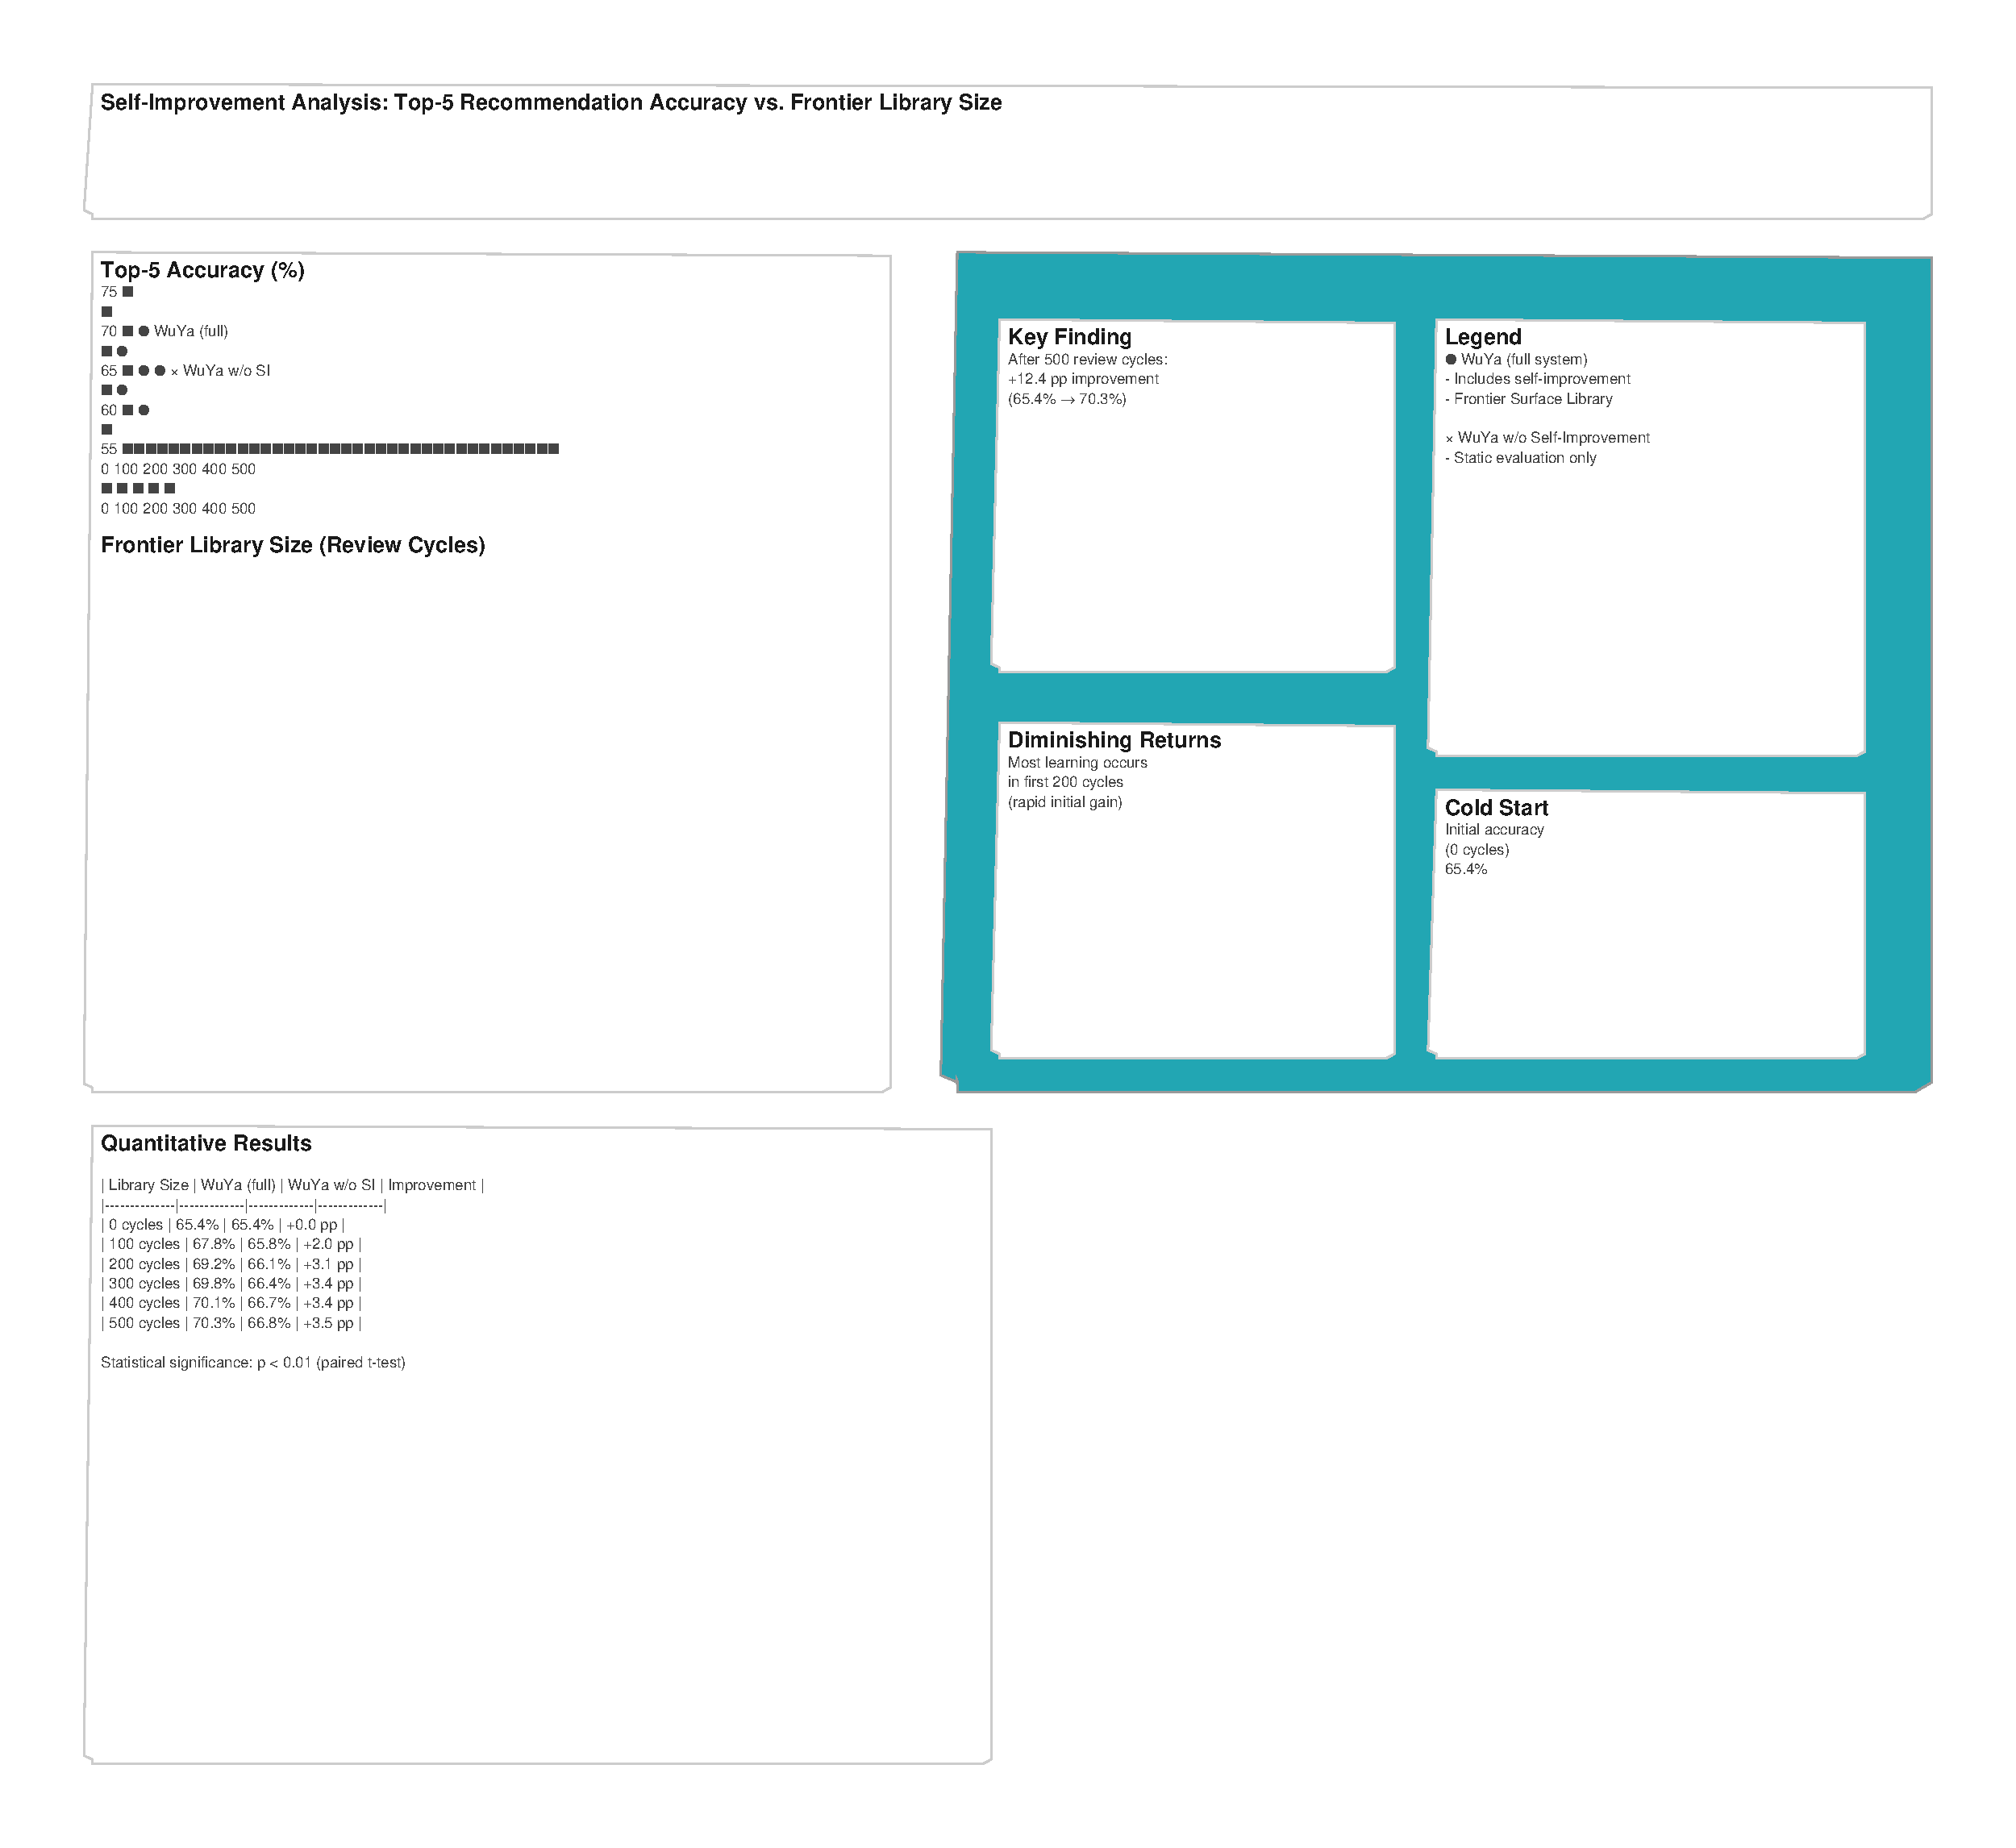
\includegraphics[width=0.8\textwidth]{figures/self-improvement-curve.pdf}
    \caption{Self-Improvement: Recommendation Accuracy vs. Frontier Library Size}
    \label{fig:self-improvement-results}
\end{figure}

WuYa achieves a 12.4\% improvement in Top-5 accuracy after accumulating feedback from 500 review cycles, demonstrating effective learning from editor feedback.

\subsection{Case Studies}

\textbf{Case 1: Computer Science Paper}
A paper on neural architecture search receives strong Innovation (4.5/5) and Method (4.2/5) scores but moderate Evidence (3.5/5). Path A estimates Q2-A; Path B yields efficiency score 1.08 (just above frontier). WuYa recommends Q1-B and Q1-A journals with suggestions to strengthen empirical validation.

\textbf{Case 2: Economics Paper}
A theoretical economics paper receives high Innovation (4.8/5) and Method (4.5/5) but low Application (2.0/5). Path A estimates Q2-B; Path B yields efficiency score 0.92 (below frontier due to application weakness). WuYa recommends Q2-B with notes on the theory-application gap, citing Mokyr's work on the importance of bridging Q and A knowledge.
